\documentclass[letterpaper,10pt,titlepage]{article}

\usepackage{graphicx}                                        
\usepackage{amssymb}                                         
\usepackage{amsmath}                                         
\usepackage{amsthm}                                          

\usepackage{alltt}                                           
\usepackage{float}
\usepackage{color}
\usepackage{url}

%\usepackage{balance}
%\usepackage[TABBOTCAP, tight]{subfigure}
%\usepackage{enumitem}
\usepackage{pstricks, pst-node}

\usepackage{geometry}
\geometry{textheight=9in, textwidth=6.5in}

%random comment

\newcommand{\cred}[1]{{\color{red}#1}}
\newcommand{\cblue}[1]{{\color{blue}#1}}

\usepackage{hyperref}
\usepackage{geometry}

\def\name{Jacob Branaugh, Brenn Kucey}

%% The following metadata will show up in the PDF properties
\hypersetup{
  colorlinks = true,
  urlcolor = black,
  pdfauthor = {\name},
  pdfkeywords = {cs472 ``computer architecture'' clements ``chapter 4''},
  pdftitle = {CS 472: Homework 4},
  pdfsubject = {CS 472: Homework 4},
  pdfpagemode = UseNone
}

\begin{document}
\hfill \name

\hfill \today

\hfill CS 472 HW 4

\begin{enumerate}
	\item[(9.2)] Why is the program counter a \textit{pointer} and not a
		\textit{counter}?
	\item[\textbullet] If the program counter was a \textit{counter}, the instructions
		would have to be sequential. Since the program counter is a
		\textit{pointer}, the instructions can be located in any order since the
		PC simply gets the next address, enabling branching.

	\item[(9.3)] Explain the function of the following registers in a CPU:
	\begin{enumerate}
		\item[-] PC (program counter): The PC holds the address of the
			\textit{next} instruction to be fetched from memory
		\item[-] MAR (memory address register): the MAR holds the address of the
			memory location that is being accessed for reading/writing during 
			the current execute cycle
		\item[-] MBR (memory buffer register): the MBR holds the data that was
			read from or is about to be written to the location pointed to by
			the address in the MAR
		\item[-] IR (instruction register): the IR holds the instruction being
			currently executed
	\end{enumerate}

	\item[(9.4)] For each of the following 6-bit operations, calculate the values of
		the C, Z, V, and N flags.
		\\
		\\
		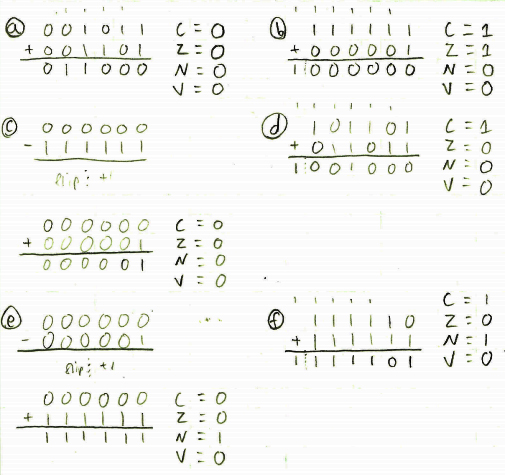
\includegraphics[scale=0.5]{problem3.jpg}

	\item[(9.5)] Why does the ARM provide a reverse subtract instruction \textit{RSB
		r0, r1, r2} that implements \textit{[r0] = [r2] - [r1]} when the normal
		subtraction instruction \textit{SUB  r0, r2, r1} will do exactly the same
		job?
	\item[\textbullet] Both operations only allow the last operand to be a flexible
		value. Flexible operands can be constants or registers with applied 
		shifts, instead of just registers. In this example, SUB allows r1 to be 
		flexible, while RSB allows r2 to be flexible. 

	\item[(9.6)] ARM instructions have a 12-bit literal. Instead of permitting a word
		in the range 0 to $2^{12}$-1, the ARM uses an 8-bit format for the integer
		and a 4-bit alignment field that allows the integer to be shifted in steps
		of 2. What are the advantages and disadvantages of this mechanism in
		comparison with a straight 12-bit integer?
	\item[\textbullet] The advantage is that the form is $(8-bit) \times  2^{4-bit}$ 
		allows for numbers larger than $2^{12}$-1. The disadvantage is that
		not all numbers between 255 and $255 \times 2^{15}$ cannot be represented 
		because not all numbers are multiples of this form.

	\item[(9.8)] Write one or more ARM instructions that will clear bits 20 to 25
		inclusive in register r0. All the other bits of r0 should remain
		unchanged.
	\item[\textbullet] AND\ \ \ r0, r0, \#0xFC0FFFFF
	\item[\textbullet] ANDS\ \ \ r0, r0, \#0xFC0FFFFF (sets status register)

	\item[(9.11)] This is a classic problem of assembly language programming. Write a
		sequence of ARM instructions that swap the contents of registers r0 and r1
		without using any additional registers or memory storage (that is, you
		can't move r1 to a temporary location).
	\item[\textbullet] This can be done using the XOR-swap algorithm:
		\begin{enumerate}
			\item[-] EOR\ \ \ r0, r0, r1
			\item[-] EOR\ \ \ r1, r0, r1
			\item[-] EOR\ \ \ r0, r0, r1
		\end{enumerate}
	\item[(9.12)] What is the binary encoding of the following instructions?
		\begin{enumerate}
			\item[a)] STRB\ \ \ r1, [r2]
			\item[-] 1110 01 0 0 0 1 0 0 0010 0001 000000000000
			\item[b)] LDR\ \ \ r3, [r4, r5]!
			\item[-] 1110 01 1 1 1 0 1 1 0100 0011 00000 00 0 0101
			\item[c)] LDR\ \ \ r3, [r4], r5
			\item[-] 1110 01 1 0 1 0 1 1 0100 0011 00000 00 0 0101
			\item[d)] LDR\ \ \ r3, [r4, \#-6]!
			\item[-] 1110 01 0 1 0 0 1 1 0100 0011 111111111010
		\end{enumerate}

	\item[(9.17)] Write an ARM assembly language program that scans a string
		terminated by the null byte 0x00 and copies the string from a source
		location pointed at by r0 to a destination pointed at by r1.
		\\
		\begin{verbatim}
		START:                  ; start of loop
		LDR   r2, [r0], #4      ; load byte into r2, increment r0 pointer
		CMP   r2, #0x00         ; check if byte is null
		BEQ   END               ; jump to end of loop if null byte
		STRB  r2, [r1], #4      ; store read byte into r1, increment r1 pointer
		B     START             ; jump to start of loop
		END:                    ; end of loop, continue with program
		\end{verbatim}

	\item[(9.22)] Write an ARM assembly language program to determine whether a string
		of characters with and odd length is a palindrome under the following
		constraints: The string of ASIC-encoded characters is stored in memory, At
		the start of the program, register r1 contains the address of the first
		character in the string, and r2 contains the address of the last
		character. On exit from the program, register r0 contains a 0 if the
		string is not a palindrome, and 1 if it is.
		\\
		\begin{verbatim}
		START:                  ; start of loop
		CMP    r1, r2           ; check if registers are pointing to same location
		MOVEQ  r0, #1           ; load immediate 1 into r0 if same location
		BEQ    END              ; jump to end of loop
		LDR    r3, [r1], #4     ; load data at location in r1 to r3, increment r1
		LDR    r4, [r2], #-4    ; load data at location in r2 to r4, decrement r2
		CMP    r3, r4           ; compare data at those locations
		MOVNE  r0, #0           ; store immediate 0 to r0 if not same character
		BNE    END              ; jump to end of loop
		B      START            ; jump to start of loop
		END:                    ; end of loop, continue with program
		\end{verbatim}
	\item[(9.23)]
	\item[(9.26)]
	\item[(9.28)]
	\item[(9.35)]
	\item[(9.41)]
	\item[(9.42)]
	\item[(9.43)]
	\item[(9.45)]
	\item[(9.46)]
	\item[(9.57)]

\end{enumerate}

\end{document}
